\section{功耗与散热管理}

在平面系统级芯片(2D SoC)中,散热通常通过散热器或基板来解决。然而,在三维集成电路(3D-IC)中,为了最大程度地缩短信号传输距离,通常需要减薄基板,这会削弱基板的传热能力。此外,由于热量可能滞留在堆叠的芯片层之间,传统的散热器方案不再是最优解。



这里介绍一种EDA生产厂商的一种功耗和散热管理的方法。在EDA生产厂商模拟SoC的功耗与发热情况是,布局规划、布局、时钟和布线是模拟流程的四个主要阶段。布局规划探索发生在流程的早期阶段,设计人员将大型功能模块放置在芯片的不同区域,确定连接方式以及模块之间的布局。在此阶段,模块具有边界,将整个芯片区域划分为粗略的区域。然后,将标准单元作为定义的模块放置在每个边界内。这些是遵循代工厂设计评审手册中规则的小型库单元。然后,它们根据本地连接通过互连进行布线。总体而言,布局规划步骤包含顶层连接的抽象视图。

\begin{figure}[htbp]
	\centering
	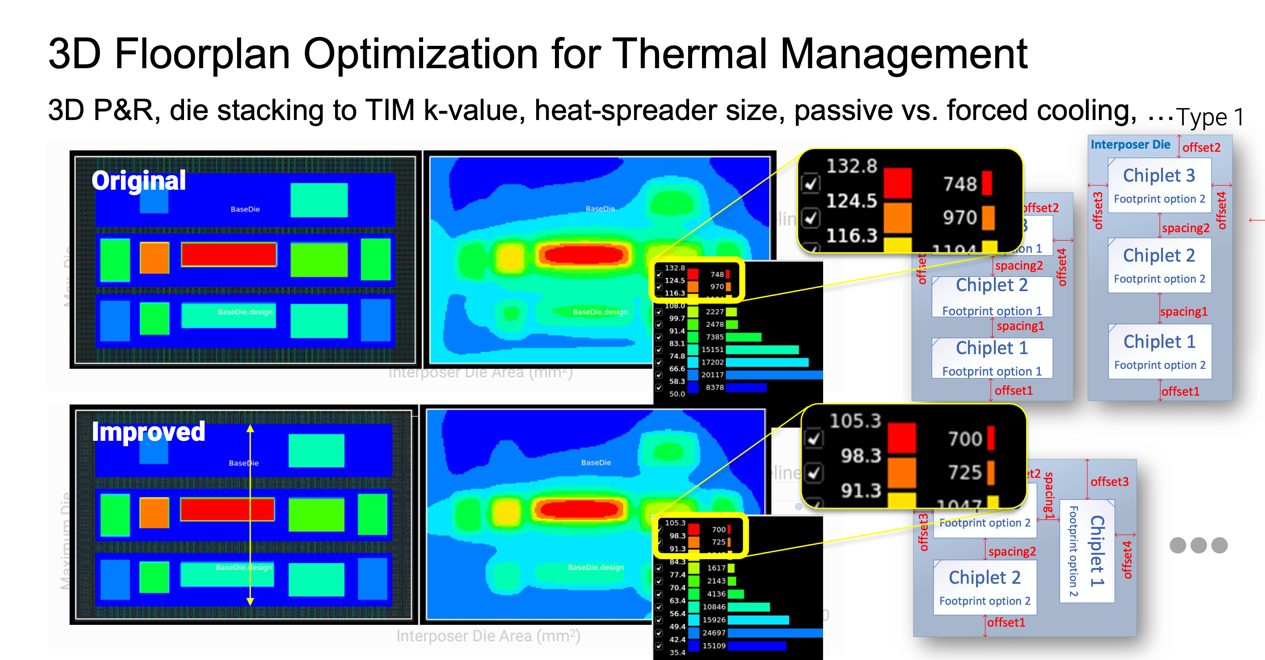
\includegraphics[width=0.8\textwidth]{img/5-1.png} % 图片文件名,不需要加扩展名
	\caption{布局规划与热管理的相互作用 \cite{Heyman2024FloorPlanning}}
	\label{fig:example}
\end{figure}

由于电压/频率调节的上下持续时间会影响性能和计算吞吐量,因此还需要进行瞬态热功率斜坡建模,并调整内部仿真温度敏感参数,例如漏电流。

集成稳压电感和用于封装设计和冷却设计的走线,系统客户还需要从芯片集设计开始的早期功率和热图,以协调组装和产品发布。因此,从寄存器传输级架构(RTL, Register-Transfer Level)之前的架构阶段到最终的流片前布局阶段 \cite{11074799},物理布局规划(包括 I/O)和一致的功率瓦特收敛也至关重要。

为了使得芯片在系统架构层面的功耗与散热管理达到一个良好的水平,需要优化芯片之间的逻辑分区。这意味着基于芯片的系统的布局布线设计流程必须考虑多芯片集成、异构技术的潜力,并管理高密度芯片间互连的复杂性。

